\section{Trajectories form regimes}

The staged quantities also support a compact regime view. We label broad-panel rows by whether they are stable-correct, stable-wrong, late-crystallizing, switch-heavy, or unstable under deterministic criteria from the cached trajectory. These labels are descriptive: they organize how the answer forms, rather than asserting a discontinuous phase transition.

\begin{figure}[tbp]
\centering
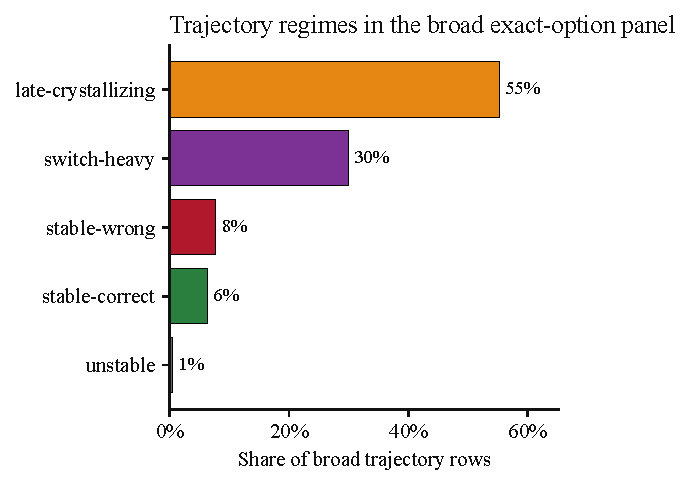
\includegraphics[width=0.96\linewidth]{figure4_regime_summary.pdf}
\vspace{0.25em}
{\small\begin{tabular}{@{}lrr@{}}
\toprule
\textbf{Trajectory regime} & \textbf{Rows} & \textbf{Share} \\
\midrule
late-crystallizing & 4924 & 55\% \\
switch-heavy & 2672 & 30\% \\
stable-wrong & 688 & 8\% \\
stable-correct & 572 & 6\% \\
unstable & 45 & 1\% \\
\bottomrule
\end{tabular}
}
\caption{\textbf{Answer-formation regimes in the broad panel.} Bars show regime shares; the table reports the exact released counts. Late-crystallizing and switch-heavy trajectories are common, showing why endpoint accuracy alone is a thin summary of answer formation.}
\label{fig:regimes}
\end{figure}

The regime view connects the staged result to heterogeneity. Some rows become stable early, some carry the correct answer late, and some continue switching leaders deep into the network. The same persistence and switch-count quantities produce all regimes, so the labels summarize trajectory shape without introducing a separate measurement target.

Across models, median $\Delta_{250}$ ranges from \MinMedianDeltaTwoFifty{} to \MaxMedianDeltaTwoFifty{}, and median write after $d_2$ ranges from \MinWriteAfterDTwo{} to \MaxWriteAfterDTwo{}. The qualitative ordering of candidate formation before winner isolation remains the common structure.
